\documentclass[11pt, a4paper]{article}

\usepackage{amsmath}
\usepackage[a4paper, margin=1in]{geometry}
\usepackage{amsfonts}
\usepackage{mathtools}

% to insert images
\usepackage{graphicx}
\graphicspath{ {./images/} {../images/}}

\usepackage{hyperref}
\hypersetup{
    colorlinks=true, % make the links colored
    linkcolor=blue, % color TOC links in blue
    urlcolor=red, % color URLs in red
    linktoc=all % 'all' will create links for everything in the TOC
}

\setlength{\parindent}{0em}

\DeclareMathOperator*{\argmin}{argmin}

\begin{document}
    %%%%%%%%%%%%%%%%%%%%%%%%%%%%%%%%%%%%%%%%%%%%%%%%%%%%%%%%%%%%%%%%%%%%%%%%%%%%%%%
    \section{Moving Beyond Linearity}
    In this section, we explore some modifications to the linear regression model in order to incorportate some non linearity as well for reducing bias/

    %%%%%%%%%%%%%%%%%%%%%%%%%%%%%%%%%%%%%%%%%%%%%%%%%%%%%%%%
    \subsection{Polynomial Regression}
    This is a simply modification to the original linear regression setting where we incorporate higher powers of the predictor as well. This helps incorporate non linear trends in the data as well while retaining an additive relationship between the variables.
    \begin{align*}
        \hat{y} &= \hat{\beta_{0}} + \hat{\beta_{1}}x \tag*{Linear Regression}\\
        \hat{y} &= \hat{\beta_{0}} + \hat{\beta_{1}}x + \hat{\beta_{2}}x^{2} + \cdots + \hat{\beta_{d}}x^{d} \tag*{Polynomial Regression}
    \end{align*}

    Generally, is is \textbf{unusual to have $d$ to be greater than $3$ or $4$} because higher degree of polynomial makes the model highly flexible with very curvy shapes. This may reduce bias to a large extent but the variance obtained thus is quite high, expecially near the end values of the range.

    \begin{align*}
        \hat{C} &= Cov(\hat{\beta}, \hat{\beta})\\
        l_{i} &= (1, x_{i}, x_{i}^{2}, \ldots, x_{i}^{d})^{T}\\
        Var[\hat{y_{i}}] &= l_{i}^{T}\hat{C}l_{i}
    \end{align*}

    The same form of polynomial regression terms works in the context of classification as well for Logistic Regression.

    
    %%%%%%%%%%%%%%%%%%%%%%%%%%%%%%%%%%%%%%%%%%%%%%%%%%%%%%%%
    \subsection{Step Function}
    Polynomial Regression, like Linear Regression, still imposes a global structure on the data. The functional form of the model is same throughout. Step Function on the other hand has a local structure and divided the range into \textbf{$k$ intervals such that each interval is fitted with a different constant}.
    \begin{align*}
        C_{0}(X) &= I(X < c_{1})\\
        C_{1}(X) &= I(c_{1} \leq X < c_{2})\\
        C_{2}(X) &= I(c_{2} \leq X < c_{3})\\
        &\hdots\\
        C_{k-1}(X) &= I(c_{k-1} \leq X < c_{k})\\
        C_{k}(X) &= I(c_{k} \geq X)\\
        \hat{y} = \beta_{0} + \beta_{1}C_{1}(x) + \cdots + \beta_{k}C_{k}(x)
    \end{align*}
    Note that, $\beta_{0}$ and $C_{0}(x)$ are equivalent since both will act as the intercept and the mean value of $y$ in the range $x < c_{1}$. Similarly, each of the $\beta_{i}$ captures the average of the response in the corresponding interval defined by the indicator function.\newline
    This approach works well when there are natural breakpoints in the data and if there are indeed constant trends in those intervals. As soon as a non constant trend emerges locally, the approach fails.

    
    %%%%%%%%%%%%%%%%%%%%%%%%%%%%%%%%%%%%%%%%%%%%%%%%%%%%%%%%
    \subsection{Basis Function}
    Basis function is the generalized form of the above two approaches. Basis are functions on $X$ that transform it. Thus, when doing regression with basis functions, we simply regress $y$ with a family of transformations of $x$.\newline
    For polynomial regression, the basis are powers of $x$ and for step function, the basis are constant values in different ranges.

    
    %%%%%%%%%%%%%%%%%%%%%%%%%%%%%%%%%%%%%%%%%%%%%%%%%%%%%%%%
    \subsection{Regression splines (Polynomials)}
    This is a class of methods that extends upon the family of polynomial and step regressions.\newline

    Instead of fitting a global polynomial to $X$, we fit \textbf{local piecewise polynomials} to X such that they are continuous at the breakpoints. The points wherer the polynomials change are called \textbf{knots}.\newline

    As we increase the number of knots, we can get a more flexible predictor. In general, if there are $K$ knots, we have $K+1$ polynomials.\newline

    Having this many splines creates a lot of degrees of freedom in the data. To solve these many equations, we need to impose constraints of \textbf{continuity and continuity of derivatives at knots}. In general, for a $d$ degree spline, we will impose the function to be continuous at knots and also have the $d-1$ derivatives to be equal at the knots. The reduced degrees of freedom are essential for obtaining unique solutions to the coefficients such that to overall curve still looks continuous.\newline

    Instead of fitting multiple splines, we can also defined the function in a single format as follows. A truncated power basis function is defined as
    \begin{align*}
        h(x, \xi) = (x - \xi)_{+}^{d} = \begin{cases} (x-\xi)^{d} &\mbox{if $x > \xi$}\\
            0 &\mbox{$0$ otherwise} \end{cases}\\
        \hat{y} = \beta_{0} + \beta_{1}b_{1}(x) + \beta_{2}b_{2}(x) + \cdots + \beta_{K+d}b_{K+d}(x)
    \end{align*}
    where the terms $b_{1},\ldots,b_{d}$ are the usual terms $x, x^{2}, \ldots, x^{d}$ and the remaining terms correspond to a truncated power function per knot. This ensures that the polynomials are continuous at the knots upto the $d-1$ derivates.\newline

    A \hypertarget{naturalsplines}{\textbf{natural spline}} is a regression spline that has the additional constraint of being linear at the boundaries, i.e., outside the extreme knots. This reduced flexibility allows for stable estimates at the knots and also makes the confidence bands narrower.

    %%%%%%%%%%%%%%%%%%%%%%%%%%%%%%%%%%%%%%%%
    \subsubsection{Choosing the degrees of freedom}
    While it may make sense to put knots at the points where the function seems to change rapidly (and not at the points where the function seems to be relatively stable), in practice the knots are usually placed at equal quantiles of the data, or generally are placed in an equidistant fashion.\newline
    For deciding the degree of freedoms, another popular choice is cross validation. We always use say $10\%$ of the data as test and gauge the RSS on this set across different degrees of freedom. A plot of RSS vs. the degrees of freedom (similar to elbow curve) can aid choosing the desired point where the RSS significantly drops.\newline
    In practice, cubic splines are popular as higher order polynomials tend to give high variance, and the plots with cubic splines also look relatively stable.


    %%%%%%%%%%%%%%%%%%%%%%%%%%%%%%%%%%%%%%%%%%%%%%%%%%%%%%%%
    \subsection{Smoothing Splines}
    The idea is to fit a smooth function that predicts the reponse well. We minimize the following
    \begin{align*}
        Loss = \sum_{i=1}^{n} (y_{i} - g(x_{i}))^{2} + \lambda \int g^{''}(t)^{2}dt \tag*{$\lambda > 0$}
    \end{align*}
    which can be decomposed into two parts, the first part encourages the function $g$ to fit the data well and the second part encourages the function to be smooth throughout.\newline
    If the function is constant or straight line, the double derivative is zero while on the other extreme, if the function changes rapidly, double derivative will also take large values.\newline

    When $\lambda$ is zero, the function simply takes the values of $y$ and thus becomes very jumpy (introducing high variance). On the other extreme, if $\lambda \to \inf$, the function is forced to be linear (which makes the double derivative zero). This is exactly the least square fit that we have seen earlier.\newline

    The function that minimizes the above loss is nothing but a cubic spline with knots at $x_{1}, x_{2}, \ldots, x_{n}$ with the additional constraint that the first and second derivatives are smooth at the knots. (The function is cubic in between the points). Outside the extreme knots, the function simply takes a linear form.\newline
    In some sense, this is similar to the \hyperlink{naturalsplines}{natural splines} but is a shrinked version of the same, $\lambda$ controlling the level of shrinkage (or how large the roughness can be).

    \begin{align*}
        \hat{g}_{\lambda} &= S_{\lambda}y\\
        df_{\lambda} &= \sum_{i=1}^{n} \{S_{\lambda}\}_{ii}
    \end{align*}
    where $\hat{g}_{\lambda}$ is a $n$-vector containing the values at the points $x_{i}$s as a solution to  a particular value of $\lambda$. $S_{\lambda}$ is a $n\times n$ matrix obtained as the solution of the above error function.

    
    %%%%%%%%%%%%%%%%%%%%%%%%%%%%%%%%%%%%%%%%
    \subsubsection{Choosing Reguularization Parameter}
    It is possible to show that as $\lambda$ increases from $0 \to \inf$, the effective degrees of freedom ($df_{\lambda}$) go from $n \to 2$.\newline

    Cross validation can also be a useful approach  to determine the value of $\lambda$. However, similar to linear regression, there exists a formula for computing the loss for LOOCV by just fitting a single model to the entire data set.
    \begin{align*}
        RSS_{cv}(\lambda) = \sum_{i=1}^{n} (y_{i} - \hat{g}_{\lambda}^{(-i)}(x_{i}))^{2} = \sum_{i=1}^{n} \bigg[ \frac{y_{i} - \hat{g}_{\lambda}(x_{i})}{1 - \{S_{\lambda}\}_{ii}} \bigg]^{2}
    \end{align*}
    where $\hat{g}_{\lambda}^{(-i)}(x_{i})$ denotes the estimate at any $x_{i}$ without using the point $i$ for calculating the loss (leave one out), while $\hat{g}_{\lambda}(x_{i})$ denotes the estimate at $x_{i}$ using all of the data.


    %%%%%%%%%%%%%%%%%%%%%%%%%%%%%%%%%%%%%%%%%%%%%%%%%%%%%%%%
    \subsection{Local Regression}
    As the name suggests, we fit regression models in the neighborhood of the point for which we want to make a prediction. But the difference from a normal linear regression is that we give weights to the points such that the points closest get higher weights and points further away get zero.\newline

    Suppose we want to make the predicton at the point $x_{0}$. The algorithm is as follows
    \begin{enumerate}
        \item gather the fraction $s = k/n$ points closest to $x_{0}$ where $s$ is also called the span an acts like a regularizer. Higher $s$ will make a global fit and vice versa.
        \item Assign a weight $K_{i0} = K(x_{i}, x_{0})$ to all the points in the neighborhood of $x_{0}$ such that the point closest gets the highest weight while the one furthest away gets the weight zero. All the other points in the data get the weight zero.
        \item Minimize the error given by
        \begin{align*}
            RSS = \sum_{i=1}^{n} K(x_{i}, x_{0})(y_{i} - \beta_{0} - \beta_{1}x_{i})^{2}
        \end{align*}
        to estimate the values of $\beta_{0}$ and $\beta_{1}$. Note that $K$ is a function known beforehand and thus constant.
        \item Make the prediction as $\hat{y}_{0} = \beta_{0} + \beta_{1}x_{0}$
    \end{enumerate}

    These models are very useful for adapting to changes in the neighborhood of a given point. The distance function can take several forms like constant, linear, quadratic or even normal distribution.\newline
    The approach can be extended to multiple dimensions as well by defining corresponding distances. However, the approach performs \textbf{poorly in dimensions higher than $3$ or $4$} as it becomes difficult to find neighbors in the surrounding area (dimensionality curse).

    
    %%%%%%%%%%%%%%%%%%%%%%%%%%%%%%%%%%%%%%%%%%%%%%%%%%%%%%%%
    \subsection{Generalized Additive Models}
    The approches discussed above are extensions of the linear regression model for a single predictor by introducing more flexbility into the models. This idea can be extended for $p$ predictors in the framework of \emph{Generalized Additive Models}. These are applicable for both classification and regression.

    \begin{align*}
        \hat{y}_{i} &= \beta_{0} + \sum_{j=1}^{p} \beta_{j} x_{ij} \tag*{Linear Rgerssion}\\
        \hat{y}_{i} &= \beta_{0} + \sum_{j=1}^{p} f_{j}(x_{ij}) \tag*{Generalized Additive Models}
    \end{align*}
    where $f_{i}(x)$ are non-linear smooth functions applied to each of the predictors separately.\newline

    Each of the functions above can be fit using all of the sections defined above. For example, some of the predictors can be smooth splines, some can be just dummy variables, and some can be polynomials. Thus, we expand from $p$ predictors to a multitude of them, where we can choose a different expansion method for each of them individually. We have combined individual simple linear regression models into a general framework for $p$ predictors.

    \begin{figure}[h]
    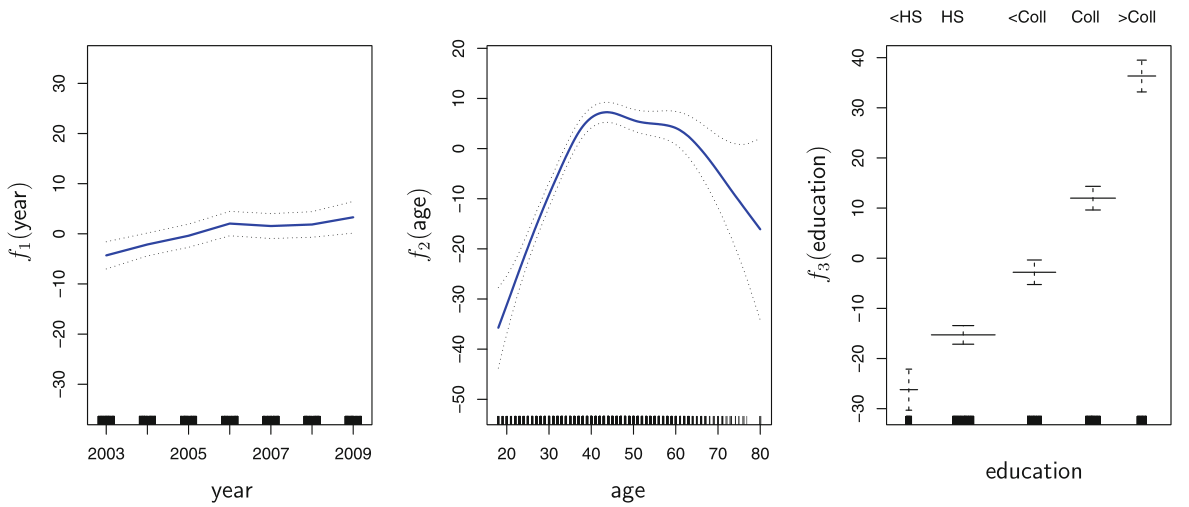
\includegraphics[scale=0.6]{gam}
    \centering
    \caption{Separate non-linear functions for three different variables. y-axis is the response. Left two plots are amoothing splines with different degrees of freedom. Right plot is dummy variables.}
    \label{fig:gam} %\ref{fig:gam}
    \end{figure}

    Fitting smoothing splines is not trivial as the loss function is not simple least squares. However, softwares can still fit using \emph{partial residuals}. We repeatedly update the fit for a single predictor, keeping the others constant.

    Summarizing,
    \begin{itemize}
        \item GAMs allow us to fit a non-linear $f_{j}$ to each $X_{j}$, so that we can automatically model non-linear relationships that standard linear regression will miss. This means that we do not need to manually try out many different transformations on each variable individually.
        \item The non-linear fits can potentially make more accurate predictions for the response $Y$ .
        \item Because the model is additive, we can still examine the effect of each $X_{j}$ on $Y$ individually while holding all of the other variables fixed. Hence if we are interested in inference, GAMs provide a useful representation.
        \item The smoothness of the function fj for the variable Xj can be summarized via degrees of freedom.
        \item The main limitation of GAMs is that the model is restricted to be additive. With many variables, important interactions can be missed. However, as with linear regression, we can manually add interaction terms to the GAM model by including additional predictors of the form $X_{j} \times X_{k}$. In addition we can add low-dimensional interaction functions of the form $f_{jk}(X_{j}, X_{k})$ into the model; such terms can be fit using two-dimensional smoothers such as local regression, or two-dimensional splines.
    \end{itemize}


    %%%%%%%%%%%%%%%%%%%%%%%%%%%%%%%%%%%%%%%%%%%%%%%%%%%%%%%%
    \subsection{Exercises}
    \begin{enumerate}
        %%%%%%%%%%Q1
        \item Suppose that a curve $\hat{g}$ is icomputed to smoothly fit a set of $n$ points using the following formula
        \begin{align*}
            \hat{g} = \argmin_{g} \bigg( \sum_{i=1}^{n} (y_{i} - g(x_{i}))^{2} + \lambda \int \big[ g^{(m)} \big]^{2} dx \bigg)
        \end{align*}
        where $g^{(m)}$ represents the $m$th derivtive of $g$ (and $g^{(0)}= g$). Provide the functional form of $g$ in the following scenarios.
        \begin{enumerate}
            \item $\lambda = \inf, m = 0$
            \item $\lambda = \inf, m = 1$
            \item $\lambda = \inf, m = 2$
            \item $\lambda = \inf, m = 3$
            \item $\lambda = 0, m = 3$
        \end{enumerate}


        %%%%%%%%%%Q2
        \item Suppose we fit a curve with basis functions $b_{1}(X) = I(0 \leq X \leq 2) - (X-1)I(1 \leq X \leq 2)$, $b_{2}(X) = (X - 3)I(3 \leq X \leq 4) + I(4 \leq X \leq 5)$. We fit the regression model
        \begin{align*}
        Y = \beta_{0} + \beta_{1}b_{1}(X) + \beta_{2}b_{2}(X) + \epsilon
        \end{align*}
        and obtain the coefficient estimates as $\hat{\beta}_{0} = 1, \hat{\beta}_{1} = 1$ and $\hat{\beta}^{2} = 3$. Plot the estimated curve between $X = -2$ and $X = 2$.
        

        %%%%%%%%%%Q3
        \item Consider the two curves $\hat{g}_{1}$ and $\hat{g}_{2}$ defined by
        \begin{align*}
            \hat{g}_{1} = \argmin_{g} \bigg( \sum_{i=1}^{n}(y_{i} - g(x_{i}))^{2} + \lambda \int \big[ g^{(3)}(x) \big]^{2} dx \bigg)
            \hat{g}_{2} = \argmin_{g} \bigg( \sum_{i=1}^{n}(y_{i} - g(x_{i}))^{2} + \lambda \int \big[ g^{(4)}(x) \big]^{2} dx \bigg)
        \end{align*}
        where $g^{(m)}$ represents the $m$th derivative of $g$.
        \begin{enumerate}
            \item as $\lambda \to \inf$, will $\hat{g}_{1}$ or $\hat{g}_{2}$ have the smaller training RSS ?
            \item as $\lambda \to \inf$, will $\hat{g}_{1}$ or $\hat{g}_{2}$ have the smaller test RSS ?
            \item as $\lambda = 0$, will $\hat{g}_{1}$ or $\hat{g}_{2}$ have the smaller training and test RSS ?
        \end{enumerate}
    \end{enumerate}


    %%%%%%%%%%%%%%%%%%%%%%%%%%%%%%%%%%%%%%%%%%%%%%%%%%%%%%%%
    \subsection{Solutions}
    \begin{enumerate}
        %%%%%%%%%%A1
        \item \label{itm:ans1} Higher derivatives will allow for a higher degree polynomial to be fit to the data
        \begin{enumerate}
            \item Since $\lambda$ is $\inf$, we only need to worry about the second term. Minimizing area under $g(x)^{2}$ is same as taking $g(x) = 0$.
            \item Similar to above, now area under $g^{(1)}(x)$ must be minimized which means the second derivative is zero and $g$ is a constant. To minimize the residuals, $g = \sum_{i=1}^{n}y_{i}$.
            \item Second derivative is zero means $g$ is a linear function. To minimize residuals, this is same as linear regression least squares.
            \item thrid derivative is zero means that $g$ is a quadratic. Hence, we fit a quadratic equation over the data by minimizing the least squares.
            \item We only need to bother with the residuals term now. Now $g$ can take many forms depending on how smooth we wish the function to be.
        \end{enumerate}
        

        %%%%%%%%%%A2
        \item For the range $[-2,2]$ the curve is simply defined as below
        \begin{alignat*}{1}
            \hat{Y} = \begin{cases} 1     &\mbox{$-2 \leq x < 0$}\\
                                    2     &\mbox{$ 0 \leq x < 1$}\\
                                    3 - x &\mbox{$ 1 \leq x \leq 2$} \end{cases}
        \end{alignat*}
        

        %%%%%%%%%%A3
        \item For $\lambda \to \inf$, the second part of the loss will dominate. As the derivative will increase, the solution can be a higher degree polynomial (as discussed in ans \ref{itm:ans1}) which means a more flexible model and hence lower error on training data.
        \begin{enumerate}
            \item $\hat{g}_{2}$ is the more flexible model and thus should have lower training RSS.
            \item Test RSS is not trivial but generally, the more flexbile the model, the higher variance it has and the lower test RSS. Thus, $\hat{g}_{1}$ should have the lower test RSS.
            \item $\lambda = 0$ implies that both the error terms are similar and thus, both the functions are same.
        \end{enumerate}
    \end{enumerate}
\end{document}